% !TeX spellcheck = en_US
\documentclass{article}
\usepackage[english]{babel}
\usepackage[utf8]{inputenc}
\usepackage{fancyhdr}
 \usepackage{xcolor}
 \usepackage{lmodern}
 \usepackage{listings}
 \lstset{language=[90]Fortran,
 	basicstyle=\ttfamily,
 	keywordstyle=\color{blue},
 	commentstyle=\color{green},
 	morecomment=[l]{!\ }% Comment only with space after !
 }
\usepackage[a4paper,left=0.7cm,right=0.7cm]{geometry}
\usepackage{wrapfig}
\usepackage{graphicx}
\usepackage{multicol}

\pagestyle{fancy}
\fancyhf{}
\lhead{Vincenzo Maria Schimmenti - 1204565}
\rhead{\today}
\rfoot{Page \thepage}
\lfoot{Exercise 3}
\title{%
	Information Theory and Computation \\
	Exercise  3}
\author{Vincenzo Maria Schimmenti - 1204565}
\begin{document}
\maketitle
 
\section*{Theory}
We rewrite a matrix multiplication program (either using different loop orders or the intrinsic Fortran function) with dynamic matrix sizing. We use a debug subroutine stored in a module for signaling possible errors or exceptions raised in the code. 
\section*{Code Development}
The matrix multiplication function has been implemented in $6$ possible ways i.e. corresponding to the possible permutation in the loop order of the matrix indices in:
\begin{equation}
	c(i,j) \leftarrow c(i,j) + a(i,k) \times b(k,j)
\end{equation}
here $a$ and $b$ are input matrices and $c$ is the resulting one; $\leftarrow$ is the assignment operator in pseudocode.
The signature of the debug subroutine is the following:
\begin{small}
	\begin{lstlisting}
	SUBROUTINE DEBUGPROC(DEBUG,CONDITION,MSG,CONTENT,FRAME,STOPONERROR)
	\end{lstlisting}
\end{small}
Here DEBUG, CONDITION,FRAME and STOPONERROR (with only the first one non-optional), MSG is a string and CONTENT is a generic scalar (an integer, a real or a logical). If DEBUG is TRUE we signal that we are in the debugging phase so in case of error we wish to get an error message; CONDITION is a logical telling whether we found an error or not: by default it is TRUE; FRAME is used to set a frame around the error message: by default is TRUE; STOPONERROR if TRUE stops the program in case of error (i.e. CONDITION is TRUE); MSG is the error message as a string; CONTENT is an optional scalar variable printed alongside the error message.
\section*{Results}
Here we show two executions of the compiled program, one without any arguments which raises an exception signaled by the framed message and one with a size of $1000$ which indeed does not raises any errors:
\begin{center}
	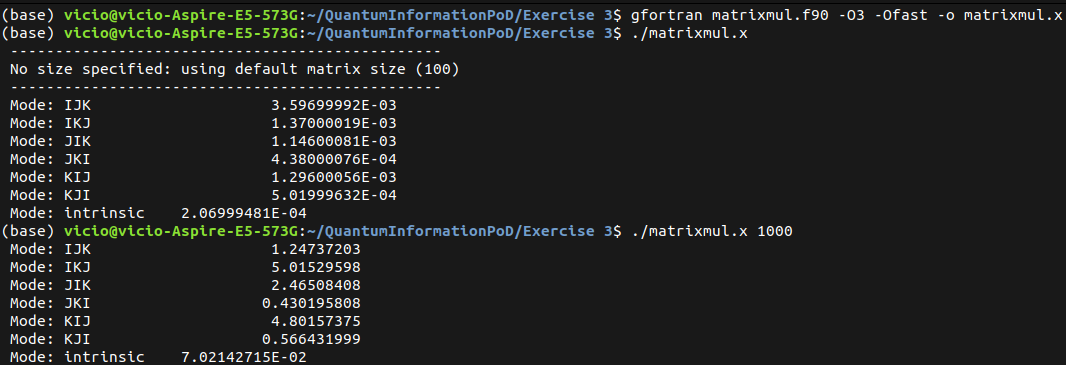
\includegraphics[width=0.65\textwidth]{Ex3.png}
\end{center}
This is done by the following piece of code:
\begin{small}
\begin{lstlisting}
debugMode = .TRUE.
if(COMMAND_ARGUMENT_COUNT() < 1)then
	call DEBUGPROC(DEBUG=debugMode,MSG="No size specified: using default matrix size (100)")
	nn = 100
else
	call GET_COMMAND_ARGUMENT(1, nnchar)
	read(nnchar,FMT=*, IOSTAT=stat)nn
	if((stat.NE.0).OR.(nn <= 0))then
	call DEBUGPROC(DEBUG=debugMode,MSG="No size specified: using default matrix size (100)")
	nn = 100
	end if
endif
\end{lstlisting}
\end{small}
Here we check for no passed argument: if so we set the use the default matrix size; if an argument is passed we try to read it into an integer: if an error is raised - either signaled by IOSTAT argument of read or by matrix size being negative - we again use the default matrix size.
\section*{Self Evalutation}
The main concern of the code was to write a good debug procedure in order to catch different possible scenarios: a good solution is provided by the generic argument CONTENT which can be of any scalar type. The debug subroutine can be further generalized in order to print vector and matrix types formatted in a readable way or to redirect the input towards a file.
\end{document}